\chapter{Introduction}

Thank you for your attendance \& welcome to the Introduction to NGS Data \& NGS Analytic Tools Workshop.
This is a free offering by the University of Adelaide, Bioinformatics Hub which is a centrally funded initiative from the Department of Vice-Chancellor (Research), with the aim of assisting \& enabling researchers in their work.
Training workshops \& seminars such as this one  are an important part of this initiative. \\

The Bioinformatics Hub itself has a web-page at \url{http://www.adelaide.edu.au/bioinformatics-hub/}, and to be kept up to date on upcoming events and workshops, please join the internal Bioinformatics mailing list on \url{http://list.adelaide.edu.au/mailman/listinfo/bioinfo}.\\

Today's workshop has been prepared with generous technical support \& advice provided by Dr Nathan Watson-Haigh (\textit{ACPFG}), Dr Dan Kortschak (\textit{Adelaide University, Adelson Research Group}), Dr Zhipeng Qu (\textit{Adelaide University, Adelson Research Group}), Dr Mark Corbett (\textit{Robinson Institute}) \& Dr John Toubia (\textit{Adelaide Centre for Cancer Genomics}). 
The tutors are Steve Pederson (\textit{Adelaide University, Bioinformatics Hub}), Dr Zhipeng Qu, \& Dr Terry Bertozzi (\textit{SA Museum \& Adelaide University, Adelson Research Group}). 
We hope it will be useful in enabling you to continue and to advance your research.\\

\section{Course Summary}
In today's workshop we will be introducing you to a small number of the basic tools required for NGS data handling, as well as giving you a basic familiarity with what the data actually looks like.
Whilst we will not be able to cover all of the rich \& diverse set of tools available, we hope to cover many of the key concepts \& questions to ask of your data, as well as give you an understanding of what information is actually in the data.\\


The majority of data handling and analysis required in the field of bioinformatics uses the \textit{command line}, alternatively known as the terminal or the \textit{bash shell}, so some useful tips for the command line will be included amongst the material.
Whilst most of the session will involve looking at individual files, in reality most of our analysis will be performed using some type of script to automate, \& easily reproduce an analysis. \\

Today's session is also intended to explore several tools in actual detail, rather than rush across the whole field.
There is large amount of information that we won't have time to discuss, but hopefully some important tools and thought processes will be covered \& enable you make better progress with your own datasets.\\

\section{Post Workshop}
The VMs which we work on today will remain active for another week after the workshop, so feel free to continue exploring any sections that you weren't able to make it through.
We'd also encourage you to sign up for some of the high-traffic websites like \textit{BioStars} or \textit{SEQanswers} as these are a rich resource for your own problem solving.


\section{Icons \& Symbols}
The following set of symbols will be used throughout this document to assist you finding your way: \\

\begin{information}
Important information.\\
\end{information}

\begin{note}
Things to note.\\
\end{note}

\begin{warning}
A warning which needs to be read very carefully.\\
\end{warning}

\begin{steps}
Instructions for you to perform. \\
\end{steps}

\begin{questions}
Questions for you to answer. \\
\begin{answer}
There is no answer
\end{answer}
\end{questions}

\begin{bonus}
An optional bonus section for those progressing rapidly. \\
\end{bonus}

\begin{advanced}
An optional advanced section for those progressing very rapidly or to be used for future reference. \\
\end{advanced}

\section{Using NoMachine} \label{sec:NoMachine}
\begin{information}
We will all be working on our own computers today, and will be accessing Virtual Machines running the Ubuntu operating system on the Nectar Research Cloud (\url{http://nectar.org.au/}).
The software client NoMachine which you will have already installed, enables us to access these machines in a familiar Desktop style, even though the majority of our time will be spent within the terminal. \\

NoMachine session files will be provided to each attendee which have been pre-configured to enable easy access to these machines.
These machines are effectively dual-core machine with 8GB of RAM \& 70GB of hard drive space.
Whilst relatively small, this will be more than enough to become familiar with the important concepts for the day.
To begin today's session, simply click (or double-click) on the NoMachine session file that you have been given.
The desktop from the Virtual Machine (VM) that you have connected to will appear on the NoMachine client. \\
\end{information}

\begin{figure}[h!]
  \centering
    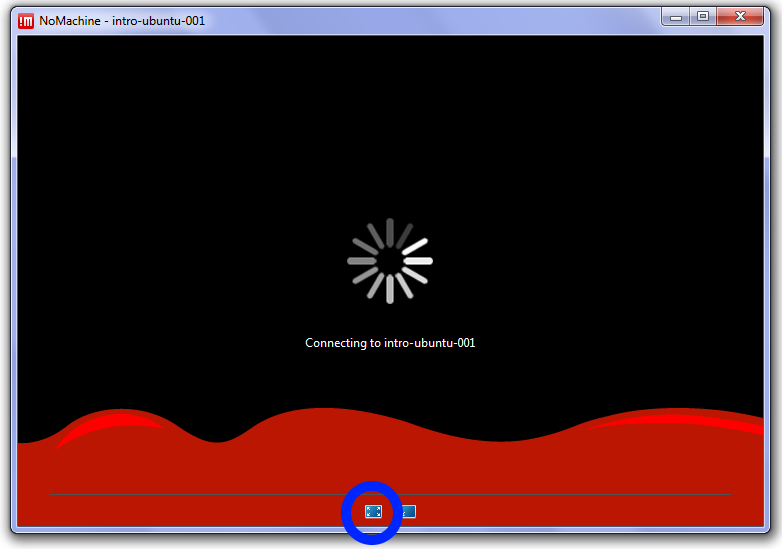
\includegraphics[width=0.8\textwidth]{NoMachine}
\end{figure}

\begin{information}
While this is connecting, select the button circled in blue above.
This will resize NoMachine to be full screen to feel more like you are physically located at the VM.
If any security warnings appear, ignore them \& continue connecting. 
It can be a little temperamental, but if connection using NoMachine fails after a few attempts, let us know \& we'll be able to get you going.\\
\end{information}

\begin{information}
Once connected to the VM, hovering your mouse over the top right corner of the screen will cause the corner of the screen to ``fold over".
If you click in the corner of this, the main control settings for NoMachine will appear.
Here you can change in \& out of the full screen setting, and you can also select the connection page to disconnect from the VM at the end of the session.
\end{information}

\section{The Ubuntu Desktop}
\begin{note}
Now that you are connected, you will notice we are in a standard graphical environment.
The default Desktop in Ubuntu is Unity, but what we are seeing is known as the Gnome Desktop.
It's easier to load this via NoMachine, but the two variants are not dissimilar.
As many of us are used to seeing, there are click-able icons on the desktop, and drop-down menus. \\

The main interfaces we will be using today are the \texttt{terminal}, a text editor named \texttt{gedit} and the web browser \texttt{firefox}
They will appear as icons on the desktop, but can also be accessed from the drop-down menus.
A \texttt{Firefox} icon is also located on the desktop \& this can be used for searching for answers as well as viewing the output of \texttt{fastqc}.
When viewing clips  you will be unable to obtain sound from the VM, so switch back to your normal laptop for these.
\end{note}

\section{Today's Data}
\begin{note}
Today we will assume a basic familiarity with the bash terminal in Linux.
Some key commands which we will be using are explained in the following table.
\end{note}
\begin{center}
  \begin{tabular}[h]{|p{3cm} | p{11.5cm} |}
    \hline
    \textbf{Command} & \textbf{Meaning} \\
    \hline
    \texttt{cd} & Change directory \\
    \texttt{ls} & List files in a directory \\
    \texttt{man} & Call the manual for a given command \\
    \texttt{head} & View the first 10 lines of a file \\
    \hline
  \end{tabular}
\end{center}

\begin{steps}
Open a terminal in the VM by either clicking on the icon, or using the drop-down menu.
It will automatically open in your home directory (\texttt{/home/trainee}), which is indicated by the tilde before the dollar sign.
The tilde (\~{}) is a symbolic representation of the address \texttt{/home/trainee}, where the first slash is the root of the file system.
To return to this directory from any other in the file system, you can simply enter the command
\begin{lstlisting}
cd 
\end{lstlisting}

Normally we specify the directory to change into after the command \texttt{cd}, but when no directory is given, this command will automatically change to your home directory.
The raw data for today's workshop is in the directory \texttt{/home/trainee/rawData}.
Change into this directory \& have a look at the files in the directory by entering the following.
\begin{lstlisting}
cd ~/rawData
ls -lhR
\end{lstlisting}
\end{steps}

\begin{warning}
Please note, the Linux operating system is case-sensitive.
When entering the above command, please make sure that you pay attention to this detail.
Spaces are an important feature as well, so be careful not to add or omit them where they appear in any sample code.
\end{warning}

After the \texttt{ls} command we specified the options \texttt{l}, \texttt{h} \& \texttt{R} by including them after the dash.
The first two of these set the output of the command to be in \textit{\underline{l}ong listing} format, and change the filesize to be output in \textit{\underline{h}uman-readable} form.
This really just means sizes are stated in Mb or Gb, instead of bytes.
You can try it without the \texttt{h} if you're curious.
The \texttt{R} option allowed the command to operate \textit{\underline{r}ecursively} through the directories within \texttt{\~{}/rawData}.
The list of options available for this command can be found using the command
\begin{lstlisting}
man ls
\end{lstlisting}
Scroll down by using the \textless \texttt{space bar}\textgreater \ until you find these two options to see what they mean.
You can navigate back a page by hitting the \textless \texttt{b}\textgreater \ key.
Exit the manual when you are finished by entering \textless \texttt{q}\textgreater.